
\documentclass[tikz]{standalone}
\usepackage{amssymb}
\usepackage{graphicx}
\usetikzlibrary{calc}
\begin{document}

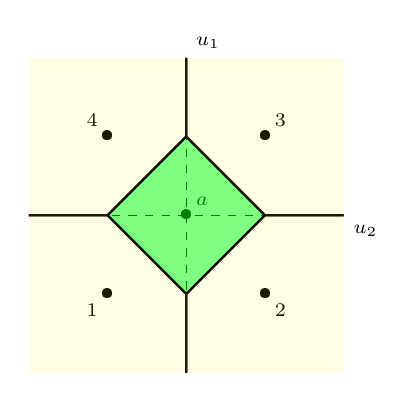
\begin{tikzpicture}
\draw[dashed] (0,-2) -- (0,2)node[anchor=south west]{\scriptsize $u_1$};
\draw[dashed] (-2,0) -- (2,0) node[anchor=north west]{\scriptsize $u_2$};

\node at (-1,-1){\textbullet} (-1,-1)node[anchor=north east]{\scriptsize $1$};
\node at (1,-1){\textbullet} (1,-1)node[anchor= north west]{\scriptsize $2$};
\node at (1,1){\textbullet} (1,1)node[anchor= south west]{\scriptsize $3$};
\node at (-1,1){\textbullet} (-1,1)node[anchor=south east]{\scriptsize $4$};
\node at (0,0){\textbullet} node[anchor=south west]{\scriptsize $a$};

\draw[thick, fill=green, opacity = 0.5] (1,0) -- (0,1) -- (-1,0) -- (0,-1) -- cycle;
\draw[thick] (2,0) -- (1,0) -- (0,1) -- (0,2);
\draw[thick] (0,2) -- (0,1) -- (-1,0) -- (-2,0);
\draw[thick] (-2,0) -- (-1,0) -- (0,-1) -- (0,-2);
\draw[thick] (0,-2) -- (0,-1) -- (1,0) -- (2,0);

\path[fill=yellow, opacity = 0.1] (2,0) -- (1,0) -- (0,1) -- (0,2) -- (2,2) -- cycle;
\path[fill=yellow, opacity = 0.1] (0,2) -- (0,1) -- (-1,0) -- (-2,0) -- (-2, 2)-- cycle;
\path[fill=yellow, opacity = 0.1] (-2,0) -- (-1,0) -- (0,-1) -- (0,-2) -- (-2,-2) -- cycle;
\path[fill=yellow, opacity = 0.1] (0,-2) -- (0,-1) -- (1,0) -- (2,0) -- (2,-2) -- cycle;

\end{tikzpicture}


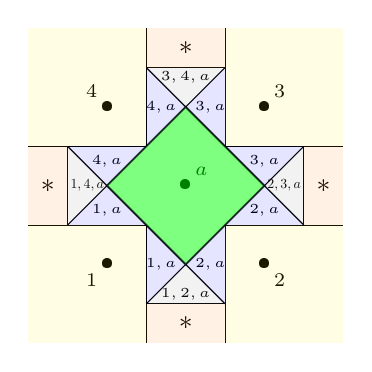
\begin{tikzpicture}
%\draw[dashed] (0,-2) -- (0,2)node[anchor=south west]{\scriptsize $u_1$};
%\draw[dashed] (-2,0) -- (2,0) node[anchor=north west]{\scriptsize $u_2$};

\node at (-1,-1){\textbullet} (-1,-1)node[anchor=north east]{\scriptsize $1$};
\node at (1,-1){\textbullet} (1,-1)node[anchor= north west]{\scriptsize $2$};
\node at (1,1){\textbullet} (1,1)node[anchor= south west]{\scriptsize $3$};
\node at (-1,1){\textbullet} (-1,1)node[anchor=south east]{\scriptsize $4$};
\node at (0,0){\textbullet} node[anchor=south west]{\scriptsize $a$};

%half lines up to sole abstain region
\draw (1/2, 2) -- (1/2, 1/2);
\draw (1/2, -1/2) -- (1/2, -2);

\draw (-1/2, 2) -- (-1/2, 1/2);
\draw (-1/2, -1/2) -- (-1/2, -2);

\draw (-2, 1/2) -- (-1/2, 1/2);
\draw (1/2, 1/2) -- (2, 1/2);

\draw (-2, -1/2) -- (-1/2, -1/2);
\draw (1/2, -1/2) -- (2, -1/2);

%lines for subsets
\draw (-3/2, -1/2) -- (1/2, 3/2);
\draw (3/2, -1/2) -- (-1/2, 3/2);
\draw (-1/2, -3/2) -- (3/2, 1/2);
\draw (-3/2, 1/2) -- (1/2, -3/2);

\draw (3/2, -1/2) -- (3/2, 1/2);
\draw (-3/2, -1/2) -- (-3/2, 1/2);
\draw (-1/2, 3/2) -- (1/2, 3/2);
\draw (-1/2, -3/2) -- (1/2, -3/2);


\path[fill=yellow, opacity = 0.1] (2,1/2) -- (1/2,1/2) -- (1/2,2) -- (2,2) -- cycle;
\path[fill=yellow, opacity = 0.1] (-1/2,2) -- (-1/2,1/2) -- (-2,1/2) -- (-2,2) -- cycle;
\path[fill=yellow, opacity = 0.1] (-2,-1/2) -- (-1/2,-1/2) -- (-1/2,-2) -- (-2,-2) -- cycle;
\path[fill=yellow, opacity = 0.1] (1/2,-2) -- (1/2,-1/2) -- (2,-1/2) -- (2,-2) -- cycle;

\draw[thick, fill=green, opacity = 0.5] (1,0) -- (0,1) -- (-1,0) -- (0,-1) -- cycle;

%mark regions where we don't have good link
\node at (-7/4, 0){$*$};
\path[fill=orange, opacity=0.1] (-2, 1/2) -- (-3/2, 1/2) -- (-3/2, -1/2) -- (-2, -1/2) -- cycle;

\node at (7/4, 0){$*$};
\path[fill=orange, opacity=0.1] (2, 1/2) -- (3/2, 1/2) -- (3/2, -1/2) -- (2, -1/2) -- cycle;
\node at (0, -7/4){$*$};
\path[fill=orange, opacity=0.1] (-1/2, -2) -- (-1/2, -3/2) -- (1/2, -3/2) -- (1/2, -2) -- cycle;
\node at (0, 7/4){$*$};
\path[fill=orange, opacity=0.1] (-1/2, 2) -- (-1/2, 3/2) -- (1/2, 3/2) -- (1/2, 2) -- cycle;

%where you have two optimal reports
\node at (-1, -5/16){\tiny$1,a$};
\path[fill=blue, opacity=0.1] (-3/2, -1/2) -- (-1,0) -- (-1/2, -1/2) -- cycle;

\node at (-5/16, -1){\tiny$1,a$};
\path[fill=blue, opacity=0.1] (-1/2, -3/2) -- (0,-1) -- (-1/2, -1/2) -- cycle;

\node at (1, -5/16){\tiny$2,a$};
\path[fill=blue, opacity=0.1] (3/2, -1/2) -- (1,0) -- (1/2, -1/2) -- cycle;

\node at (5/16, -1){\tiny$2,a$};
\path[fill=blue, opacity=0.1] (1/2, -3/2) -- (0,-1) -- (1/2, -1/2) -- cycle;

\node at (5/16, 1){\tiny$3,a$};
\path[fill=blue, opacity=0.1] (1/2, 3/2) -- (0,1) -- (1/2, 1/2) -- cycle;

\node at (1, 5/16){\tiny$3,a$};
\path[fill=blue, opacity=0.1] (3/2, 1/2) -- (1,0) -- (1/2, 1/2) -- cycle;

\node at (-1, 5/16){\tiny$4,a$};
\path[fill=blue, opacity=0.1] (-3/2, 1/2) -- (-1,0) -- (-1/2, 1/2) -- cycle;

\node at (-5/16, 1){\tiny$4,a$};
\path[fill=blue, opacity=0.1] (-1/2, 3/2) -- (0,1) -- (-1/2, 1/2) -- cycle;

%three optimal reports
\node at (0, -11/8){\tiny$1,2,a$};
\path[fill=gray, opacity=0.1] (-1/2, -3/2) -- (0,-1) -- (1/2, -3/2) -- cycle;

\node at (-5/4,0){\scalebox{0.5}{$1,4,a$}};
\path[fill=gray, opacity=0.1] (-3/2, -1/2) -- (-1,0) -- (-3/2, 1/2) -- cycle;

\node at (5/4,0){\scalebox{0.5}{$2,3,a$}};
\path[fill=gray, opacity=0.1] (3/2, -1/2) -- (1,0) -- (3/2, 1/2) -- cycle;

\node at (0, 11/8){\tiny$3,4,a$};
\path[fill=gray, opacity=0.1] (-1/2, 3/2) -- (0,1) -- (1/2, 3/2) -- cycle;

\end{tikzpicture}

\end{document}
%%% Local Variables:
%%% mode: latex
%%% TeX-master: t
%%% End:
